% !TeX spellcheck = fr_FR
\chapter{Chapitre 2 : Algorithmes}

Ce chapitre contient les différents algorithme rencontré lors de l'application 

\section{Nettoyage}

L'utilité de réduire la quantité de données sauvegardées de nos jours au vu des 
moyens de stockage moderne employés n'est plus une occupation majeure.
Cependant, certains systèmes d'informations restent limités en mémoire et en
puissance de calcul notamment les smartphones ou encore les ordinateurs portable.
Dans ces cas, 
% c'est à ce moment qu'intervient un nettoyage de données.
Le nettoyage des données \gls{lidar} est aussi utile sur des systèmes plus puissants
pour accélérer l'utilisation ultérieure des fichiers par la quantité réduite
d'information.
Les méthodes présentées ici ne sont pas exhaustive et peuvent être utilisées
de manière indépendante ou bien combinées ensemble.

\subsection{Lidar}

Les données brutes provenant des instruments \gls{lidar} contiennent souvent
des informations bruitées et inutile. Ces dernières peuvent fausser les résultats
finaux et prennent de la mémoire de stockage supplémentaire.

\subsubsection{Nettoyage par point pondéré}

Une autre manière de réduire la quantité de données est de remplacer plusieurs points par un seul où l'élévation de celui-ci équivaut à la moyenne des élévations des voisins.
En d'autres termes $$ P_{\bar{y}} = \frac{1}{n} \sum_{i=0}^{n} p_{iy} $$
où $n$ est le nombre de voisins d'un point $P$. 
Le choix de l'endroit où l'on créera le point peut être déterminé à l'aide d'une condition, p. ex. $$\sum_{i=0}^n dist(P, p_i) \geq \epsilon$$

Un effet de bord de cette méthode est le lissage des surfaces plates. Un exemple serait les illustrations \ref{fig:before_las_filter} et \ref{fig:after_las_filter} où l'on peut observer qu'après une reconstruction de surface, on aperçoit que les points on une tendance à moins osciller dans l'axe vertical.
\begin{figure}[htbp!]
    \centering
    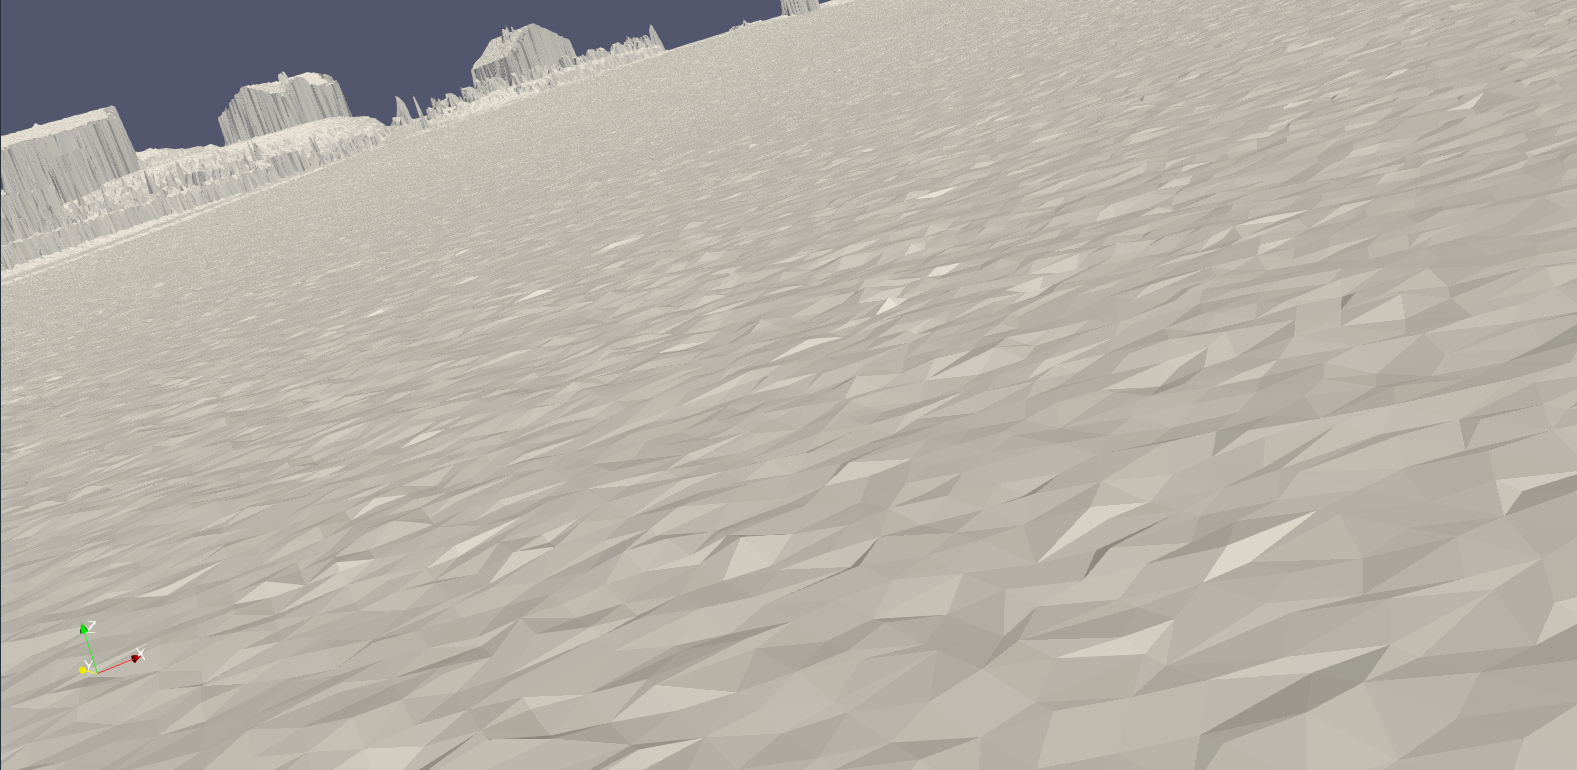
\includegraphics[width=0.8\linewidth]{figures/lissage_brut.png}
    \caption{Surface plane avant le nettoyage. Source : réalisé par Jérôme Chételat}
    \label{fig:before_las_filter}
\end{figure}
\begin{figure}[htbp!]
    \centering
    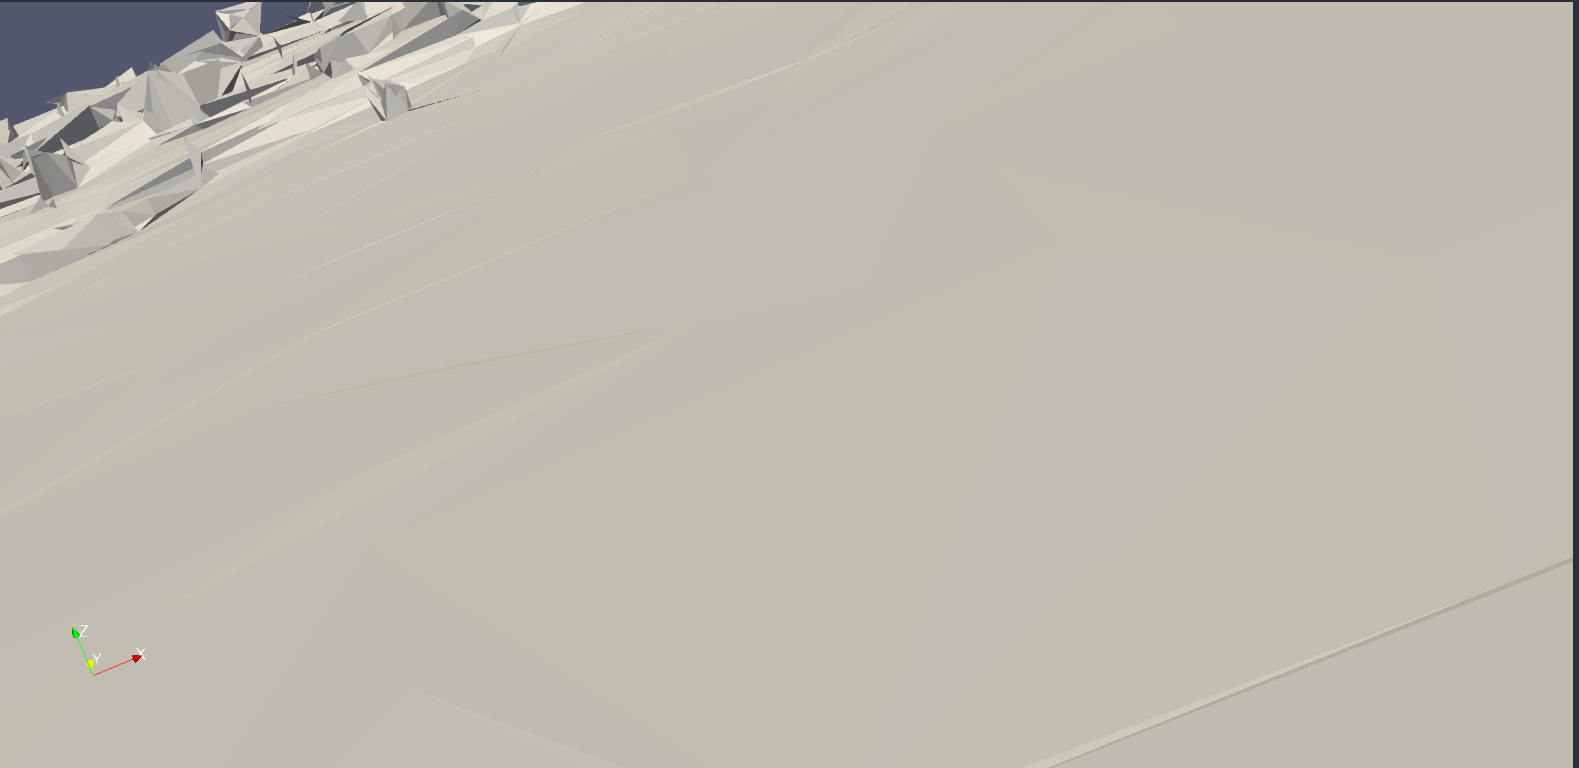
\includegraphics[width=0.8\linewidth]{figures/lissage_filtrer.png}
    \caption{Surface plane après le nettoyage. Source : réalisé par Jérôme Chételat}
    \label{fig:after_las_filter}
\end{figure}

\subsubsection{Nettoyage par point moyen}

Ce filtre se base sur l'utilisation de l'intensité de retour d'une impulsion. Les points à retour multiple peuvent être nombreux en présence d'arbres. Au lieu d'avoir plusieurs points de retour, on les remplace par un seul point qui prend une moyenne de toutes les positions de retour de la même impulsion. En terme mathématique, on a donc : 
$$
P = 
\begin{pmatrix}
    \bar{x} \\
    \bar{y} \\
    \bar{z}
\end{pmatrix}
=
\frac{1}{n}
\sum_{i=0}^{n}
\begin{pmatrix}
   p_{i_x} \\
   p_{iy} \\
   p_{iz} \\
\end{pmatrix}
$$

Où $n$ désigne le nombre de retour d'une impulsion et $p$ les points de l'impulsion.

\subsubsection{Nettoyage par classe de point lidar}

Une méthode différente pour nettoyer les données est de se baser sur la 
classification des points présentée au chapitre 1.1.
En connaissant le type de points qui nous intéresse, il est possible de charger
en mémoire uniquement le ou les types de points voulus. 
% En connaissant les informations qui nous intéressent, le nettoyage se fait 
% donc lors de la lecture des données.
% Étant donné que la lecture se déroule de manière séquentielle, il suffit de
% poser une ou plusieurs conditions vérifiant la classe du point.

La manière de procéder est la suivante.
Lors de la lecture du fichier lidar, la catégorie du point est testée.

Une fois la lecture terminée, on réécrit la liste des points gardés dans un nouveau fichier \gls{lidar}.
Le fichier original peut être supprimé ou conservé.


\subsection{Maillage}
On appelle maillage le résultat d'une reconstruction de surface. On peut aussi
l'appeler triangulation.

\subsection{Nettoyage de maillage}

Le nettoyage de maillage repose sur le principe de la hauteur moyenne des
voisins.

\section{Triangulation de Delaunay}
Dans cette section, on détail les algorithme de reconstruction de surface.
Il existe plusieurs manière de créer le même résultat mais une méthode utilisée est la triangulation de Delaunay.
La triangulation de Delaunay est une manière de créer des triangles entre des points dispersés dans l’espace.
Cette manière de trianguler les points permet de créer un résultat plus homogène que d’autres méthodes.
On peut observer des résultats différents dans la figure
\ref{fig:triangulation_example}

\begin{figure}[htb!]
    \centering
    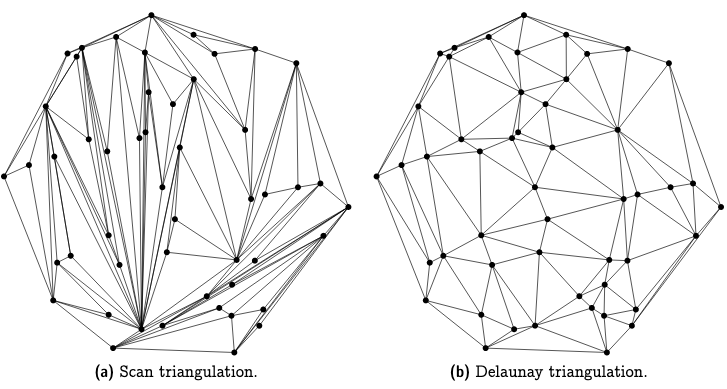
\includegraphics[width=0.8\linewidth]{figures/triangulation-example.png}
    \caption{Deux triangulations appliquées sur même jeu de données. Source : tiré de ref URL01}
    \label{fig:triangulation_example}
\end{figure}

\subsection{Bowyer-Watson}
L'algorithme de Bowyer-Watson est conceptuellement simple.
C'est un algorithme itératif découvert par Adrian Bowyer et David Watson.
Le principe de ce dernier repose sur l’ajout progressif de points dans la triangulation.
Après chaque ajout, de nouveaux triangles sont formés à partir du point ajouté et des sommets du triangle contenant le point.

Soit $\mathcal{P} \subset \mathbb{R}^2$ l'ensemble des points à trianguler et $\mathcal{T}$ les triangles appartenant à la triangulation.
On construit dans un premier temps, un triangle $S \in \mathcal{T}$ tel que $\mathcal{P} \subset S$.
On nomme ce triangle le "super-triangle".
Il doit contenir en son sein l'ensemble des points $\mathcal{P}$. On ajoute donc trois points, les sommets de $S$ dans $\mathcal{P}$.

\begin{figure}[htbp!]
    \centering
    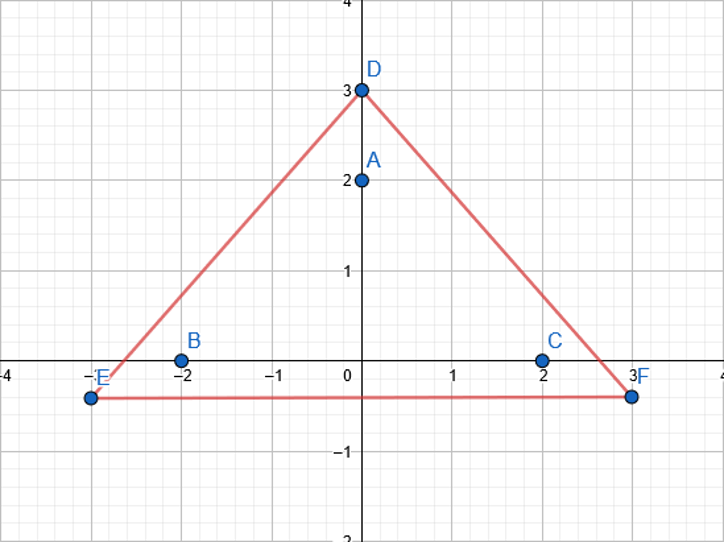
\includegraphics[width=0.66\linewidth]{figures/bowyer-watson/step_3.png}
	\caption{Création du super-triangle englobant l'ensemble de points $\mathcal{P}$. Source : réalisé par
	Jérôme Chételat}
	\label{fig:triangulation_step_3}
\end{figure}

On prend ensuite un point de $\mathcal{P}$ puis on détermine dans quel triangle il se situe.
Pour connaître l'appartenance d'un point dans un triangle, on détermine si un point est contenu dans le cercle circonscrit dudit triangle.
La condition qui permet de déterminer si un point $D$ est contenu dans le cercle-circonscris de $\triangle ABC$ est la suivante :

\begin{figure}[htbp!]
    \centering
    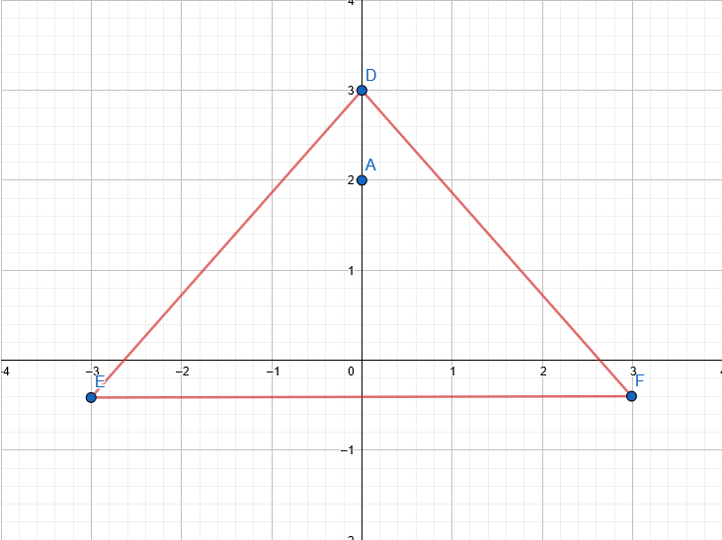
\includegraphics[width=0.66\linewidth]{figures/bowyer-watson/step_4.png}
    \caption{Ajout du premier points de dans la triangulation. Source : réalisé par
	Jérôme Chételat}
	\label{fig:triangulation_step_4}
\end{figure}





$$
\begin{vmatrix}
 A_x - D_x & A_y - D_y & (A_x - D_x)^2 + (A_y - D_y)^2 \\
 B_x - D_x & B_y - D_y & (B_x - D_x)^2 + (B_y - D_y)^2 \\
 C_x - D_x & C_y - D_y & (C_x - D_x)^2 + (C_y - D_y)^2 \\
\end{vmatrix} \geqslant 0
$$

Si la condition est vraie, le point est relié au sommet du triangle qui le contient.
Les arrête créées forment de nouveaux triangles appartenant désormais à la
triangulation $\mathcal{T}$. Dans le cas de la première itération, on a le
résultat intermédiaire dans la figure \ref{fig:triangulation_step_5}.

\begin{figure}[htbp!]
    \centering
    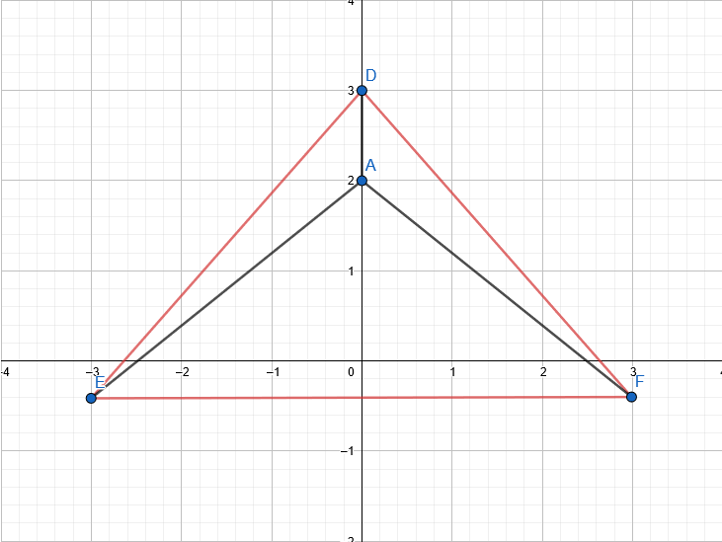
\includegraphics[width=0.66\linewidth]{figures/bowyer-watson/step_5.png}
    \caption{Ajout des arrêtes reliant les sommets du super-triangle au point
		ajouté dans la triangulation. Source : réalisé par
	Jérôme Chételat}
	\label{fig:triangulation_step_5}
\end{figure}

On répète les opérations d'ajout de points et de création de triangles jusqu'à ce qu'on ait parcouru tous les points de $P$

Pour finir, on identifie les arrêtes reliées aux sommets du super-triangle puis on
les supprime de la triangulation $\mathcal{T}$.
On supprime également les sommets du super-triangle ainsi que ses arrêtes de 
$\mathcal{P}$ et de $\mathcal{T}$. 

Le résultat est un ensemble de triangles $\mathcal{T}$ représentant la géométrie
des surfaces. Cette dernière est appelée triangulation de Delaunay.
Ce résultat est unique pour un ensemble de points $\mathcal{P}$ donné.
Voici un exemple de triangulation finale dans la figure \ref{fig:example_delaunay}.

\begin{figure}[htbp!]
    \centering
    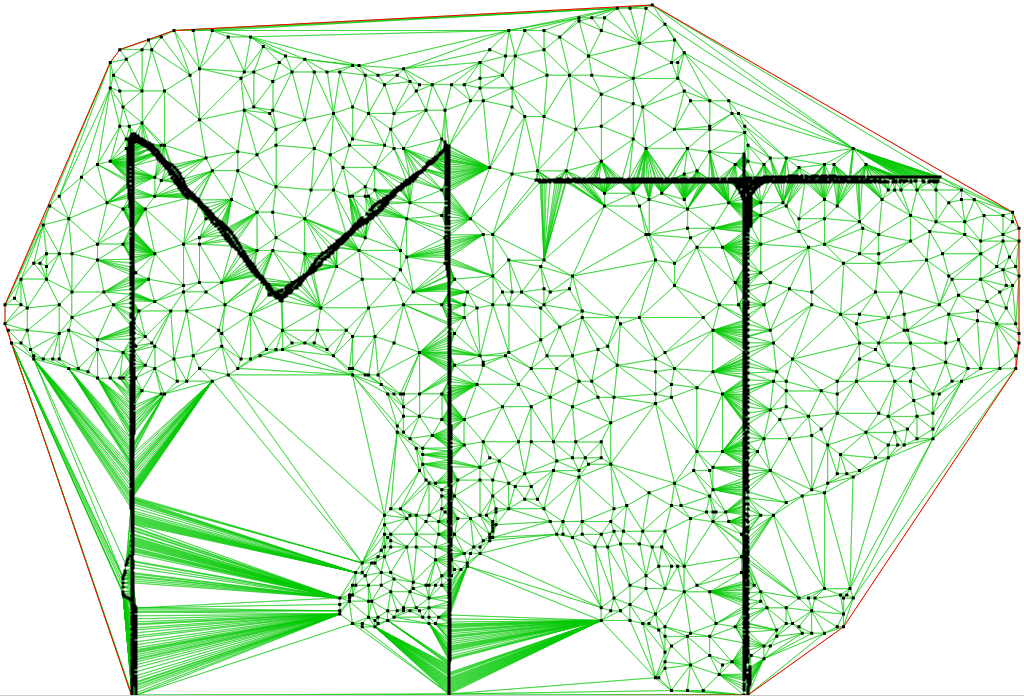
\includegraphics[width=0.8\linewidth]{figures/example_delaunay.png}
    \caption{Maillage résultant d'une triangulation de delaunay. Source : réalisé par Jérôme Chételat}
    \label{fig:example_delaunay}
\end{figure}

\subsection{Lee \& Scachter}

L'algorithme de Lee et Scachter est basé sur le principe de "Divide and conquer".
Le principe consiste à former des petites triangulations à partir d'un espace divisé selon un axe.
On applique une triangulation pour la première itération.
Ensuite, on fusionne les triangulations entre elles et l'on répète ces étapes jusqu'à ne plus pouvoir en fusionner.
Le résultat final est un maillage considéré comme étant triangulation de Delaunay. 

\section{Fusion de maillage}

L'algorithme présenté dans cette section concerne la fusion de maillage.
Dans l'application du travail de bachelor, il se peut que l'on ait déjà des triangulations existantes et que l'on souhaite afficher un résultat de la fusion des deux triangulations.
Il s'agit en réalité que d'une partie de l'algorithme de triangulation par Lee et Scachter basé sur le principe de "Divide and conquer".

Soit deux triangulations $M_L$ et $M_R$ linéairement séparable par une droite $g$.
On cherche en premier les sites aux extrémités inférieures selon l'axe $y$ et on les relie par une arrête coupant la droite $g$.
L'arrête créée est nommée "base LR". On a donc une situation similaire à l'illustration \ref{fig:base_lr}

\begin{figure}[!htb]
    \centering
    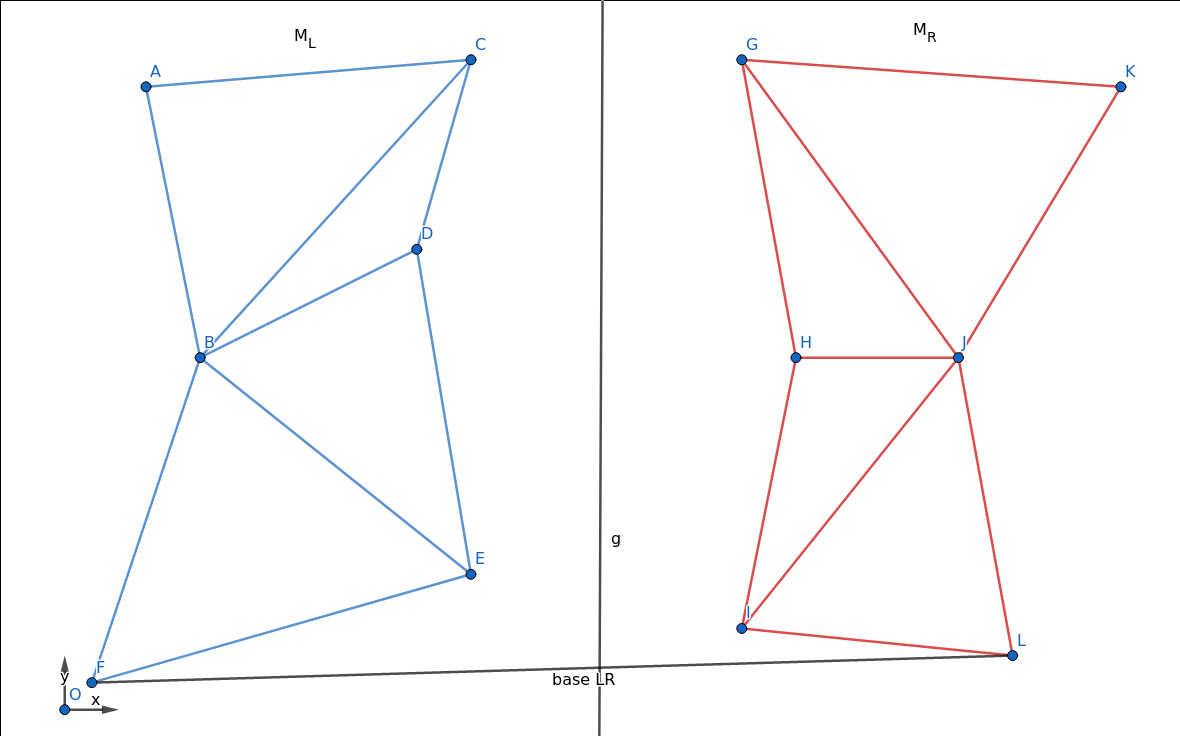
\includegraphics[width=0.8\linewidth]{figures/base_lr.png}
    \caption{Création de la base LR entre les deux maillages. Source: réalisé par Jérôme Chételat}
    \label{fig:base_lr}
\end{figure}

On poursuit par la recherche d'un site candidat voisin d'une des extrémités de la base LR qui respecte les conditions suivantes:

\begin{enumerate}
    \item L'angle ,dans le sens antihoraire pour un site de $M_R$ et dans le sens horaire pour un site de $M_L$, par rapport à la base LR est inférieur à 180°.
    \item Le cercle circonscrit défini par les deux extrémités de la base et l'une des extrémités avec un candidat ne contient pas un prochain candidat potentiel en son sein.
\end{enumerate}

Si les deux conditions sont satisfaites, le site devient un candidat final pour le maillage en question.
Si la première condition n'est pas respectée, aucun candidat pour le maillage n'est choisi et l'arrête reliant le candidat actuel avec la base est supprimé de la triangulation.

Le processus de choix d'un candidat se poursuit tant qu'aucun candidat final ne soit choisi ou qu'on détermine qu'aucun candidat ne peut être choisi.

Les illustrations \ref{fig:site_ML_candidate} et \ref{fig:site_MR_candidate} représente le choix d'un candidat final pour chaque maillage. Cela ne représente que la première itération.
\begin{figure}[htbp!]
    \centering
    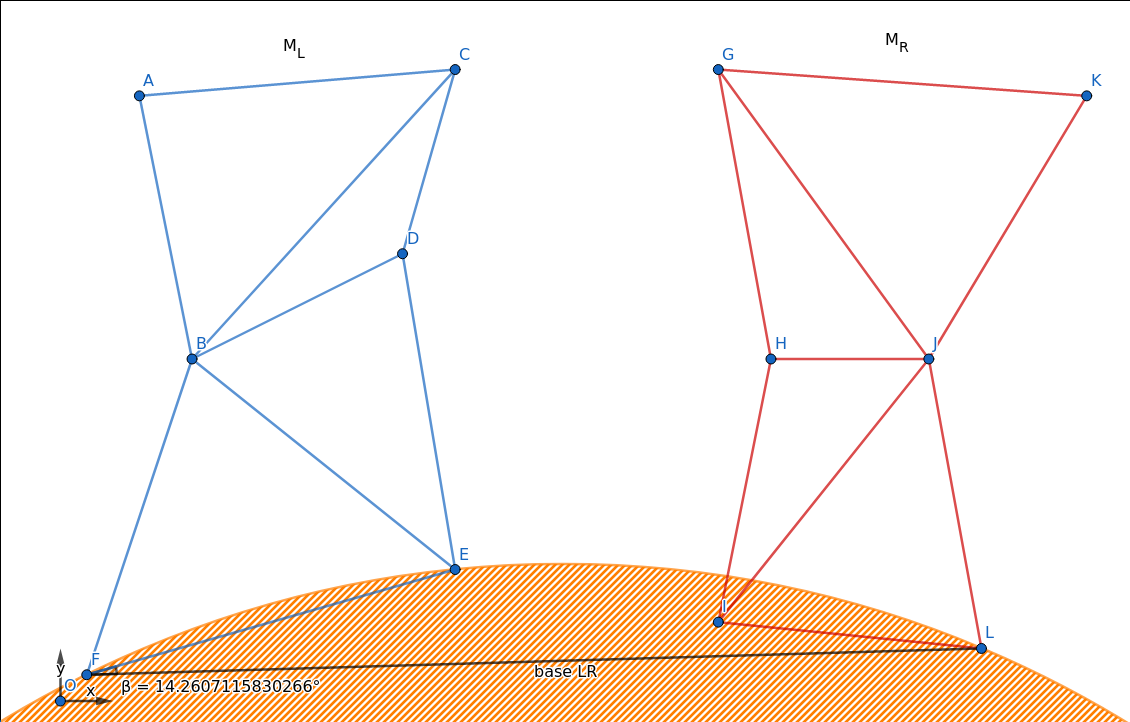
\includegraphics[width=0.8\linewidth]{figures/site_ML.png}
    \caption{Candidat final du maillage $M_L$. Source: réalisé par Jérôme Chételat}
    \label{fig:site_ML_candidate}
\end{figure}

\begin{figure}[htpb!]
    \centering
    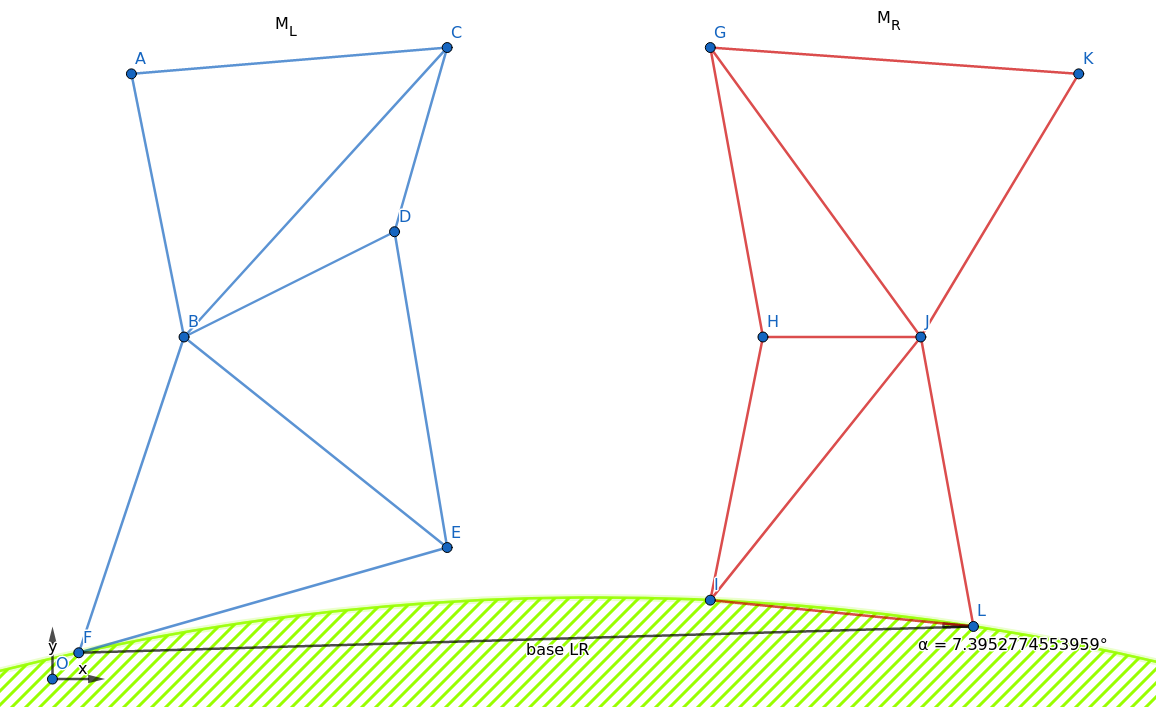
\includegraphics[width=0.8\linewidth]{figures/site_MR.png}
    \caption{Candidat final du maillage $M_R$. Source: réalisé par Jérôme Chételat}
    \label{fig:site_MR_candidate}
\end{figure}

Une fois que les candidats pour chaque maillage ont été déterminés, si un seul candidat final est présent, on lie le candidat par une arête avec le site de la base du maillage opposé. Dans le cas où deux candidats sont choisis, on détermine un dernier test. On vérifie qu'un candidat final n'est pas contenu dans le cercle circonscrit de l'autre. Si c'est le cas, le candidat qui contient le site dans le cercle circonscrit est alors abandonné et celui qui n'en contient pas est utilisé pour créer une nouvelle base. On peut observer que dans le la figure \ref{fig:site_ML_candidate} le site $I$ est contenus dans le cercle circonscrit formé par les points $F, E$ et $L$. Dans ce cas, le site $E$ n'est pas maintenu en tant que candidat final et une arrête entre $I$ et $F$ est créée. Celle-ci devient alors la nouvelle base.

Les opérations de recherche de candidat et de création d'arêtes continuent jusqu'à ce que plus aucun candidat final ne soit obtenu.
